% --- Use 'standalone' class to crop the output to the figure ---
\documentclass[tikz, border=10pt]{standalone}

% --- Load TikZ Libraries ---
\usepackage{tikz}
\usetikzlibrary{arrows.meta, positioning}
\usepackage{amsmath} % For math environments like \frac

% --- Color Definitions ---
\definecolor{VectorColor}{RGB}{45, 114, 178}
\definecolor{PointColor}{RGB}{213, 94, 0}
% AxisColor removed, using black for axes

\begin{document}

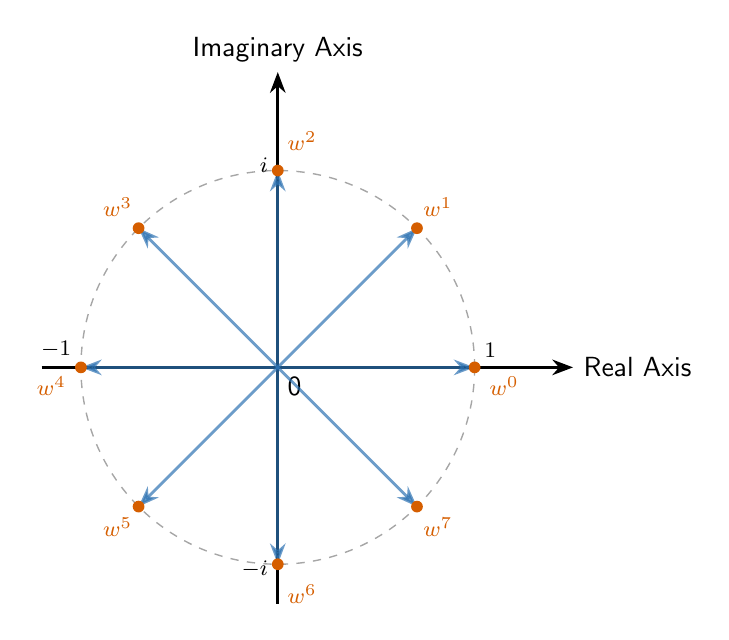
\begin{tikzpicture}[
    font=\sffamily,
    >=Stealth,
    scale=2.5, % Increased scale for better visibility
    root/.style={circle, fill=PointColor, inner sep=1.5pt} % Style for the root points
]

% --- Draw Axes (Complex Plane) - Black ---
\draw[->, black, line width=1pt] (-1.2, 0) -- (1.5, 0) node[right] {Real Axis};
\draw[->, black, line width=1pt] (0, -1.2) -- (0, 1.5) node[above] {Imaginary Axis};

% --- Draw the Unit Circle (dashed gray) ---
\draw[gray!70, dashed, line width=0.5pt] (0, 0) circle (1.0);
\node[below right] at (0, 0) {0};

% --- Separate Labels for Cardinal Points (1, -1, i, -i) ---
% MODIFIED: Label '1' is now positioned above the axis
\node[above right, font=\footnotesize] at (1, 0) {$1$};
\node[above left, font=\footnotesize] at (-1, 0) {$-1$};
\node[left, font=\footnotesize, yshift=2pt] at (0, 1) {$i$};
\node[left, font=\footnotesize, yshift=-2pt] at (0, -1) {$-i$};


% --- Loop to Draw the 8 Roots of Unity ---
\foreach \k in {0,...,7}
{
    \pgfmathsetmacro{\angle}{45 * \k} % Angle step is 45 degrees.
    
    % Draw the vector from the origin to the root
    \draw[->, VectorColor, line width=1pt, opacity=0.7] (0, 0) -- (\angle:1);

    % Draw the root point (node)
    % All points use the 'root' style, ensuring consistent size
    \node[root] at (\angle:1) {};
    
    % --- Conditional Labeling for w^k ---
    % Radial distance for all labels is now 1.15 (just outside the circle point)
    \pgfmathsetmacro{\radialdist}{1.15}
    
    \ifnum\k=0 % 1 (Real Axis - Right)
        % Positioned at 1.15 radial distance, below the x-axis (to avoid '1' label which is now above)
        \node[PointColor, font=\footnotesize, below] at (\radialdist, 0) {$w^0$};
    \else\ifnum\k=2 % i (Imaginary Axis - Up)
        % Positioned at 1.15 radial distance, right of the y-axis (to avoid 'i' label)
        \node[PointColor, font=\footnotesize, right] at (0, \radialdist) {$w^2$};
    \else\ifnum\k=4 % -1 (Real Axis - Left)
        % Positioned at 1.15 radial distance, below the x-axis (to avoid '-1' label)
        \node[PointColor, font=\footnotesize, below] at (-\radialdist, 0) {$w^4$};
    \else\ifnum\k=6 % -i (Imaginary Axis - Down)
        % Positioned at 1.15 radial distance, right of the y-axis (to avoid '-i' label)
        \node[PointColor, font=\footnotesize, right] at (0, -\radialdist) {$w^6$};
    \else
        % For non-cardinal roots (1, 3, 5, 7), place the label at 1.15 along the vector (up the vector)
        \node[PointColor, font=\footnotesize] at (\angle:\radialdist) {$w^{\k}$};
    \fi\fi\fi\fi
}

\end{tikzpicture}

\end{document}